\documentclass[aspectratio=169]{beamer}
\usepackage[utf8]{inputenc}
\usepackage[T1]{fontenc}
\usepackage[brazil]{babel}
\usepackage{ragged2e}
\usepackage{booktabs}
\usepackage{verbatim}
\usepackage{gensymb}
\usepackage{multirow}
\usepackage{xcolor,colortbl}
\definecolor{verde}{rgb}{0,0.5,0}
\usepackage{listings}
\lstset{
  language=C++,
  basicstyle=\ttfamily\small,
  keywordstyle=\color{blue},
  stringstyle=\color{verde},
  commentstyle=\color{red},
  extendedchars=true,
  showspaces=false,
  showstringspaces=false,
%  numbers=left,
%  numberstyle=\tiny,
  breaklines=true,
  backgroundcolor=\color{green!10},
  breakautoindent=true,
  captionpos=b,
  xleftmargin=0pt
}
\newcommand\setItemnumber[1]{\setcounter{enumi}{\numexpr#1-1\relax}}

\usetheme{AnnArbor}
\usecolortheme{orchid}
\usefonttheme[onlymath]{serif}

\AtBeginSection[]{
  \begin{frame}
  \vfill
  \centering
  \begin{beamercolorbox}[sep=8pt,center,shadow=true,rounded=true]{title}
    \usebeamerfont{title}\insertsectionhead\par%
  \end{beamercolorbox}
  \vfill
  \end{frame}
}

\title[\sc{Composição}]{Composição}
\author[Roland Teodorowitsch]{Roland Teodorowitsch}
%\institute[LP2 - EC - PUCRS]{Laboratório de Programação II - Curso de Engenharia de Computação - PUCRS}
\institute[POO - EC - PUCRS]{Programação Orientada a Objetos - ECo - Curso de Engenharia de Computação - PUCRS}
\date{30 de agosto de 2023}

\begin{document}
\justifying

%-------------------------------------------------------
\begin{frame}
	\titlepage
\end{frame}

%=======================================================
\section{Composição}

%-------------------------------------------------------
\begin{frame}\frametitle{Conceito de Composição}
\begin{itemize}
	\item Objetos fazendo parte de outros objetos
	\item Princípio básico da engenharia de software
	\begin{itemize}
		\item Módulos menores fazem parte de módulos maiores
	\end{itemize}
	\item Exemplo:
	\begin{itemize}
		\item Carro
		\begin{itemize}
			\item Motor: um carro possui um motor
			\item Pneus[4]: Um carro possui quatro rodas com pneus
		\end{itemize}
	\end{itemize}
\end{itemize}
\end{frame}

%-------------------------------------------------------
\begin{frame}\frametitle{Funcionamento da Composição}
\begin{itemize}
	\item Objetos membros inicializados antes dos objetos de que fazem parte
	\begin{itemize}
		\item Pode-se explorar os métodos construtores para inicialização.
	\end{itemize}
	\item Exemplo:
	\begin{itemize}
		\item Um produto com data de validade
		\begin{itemize}
			\item Data de validade é um atributo da classe \texttt{Produto}
			\item ... Mas data de validade também é um objeto da classe \texttt{Data}
			\item Desta forma, pode-se dizer que produto depende de \texttt{Data}
			\item Ou seja, \texttt{Produto} utiliza os ``serviços'' da classe \texttt{Data}
		\end{itemize}
	\end{itemize}
\end{itemize}
\end{frame}

%-------------------------------------------------------
\begin{frame}\frametitle{Exemplo}
\begin{figure}[h]
	\centering
	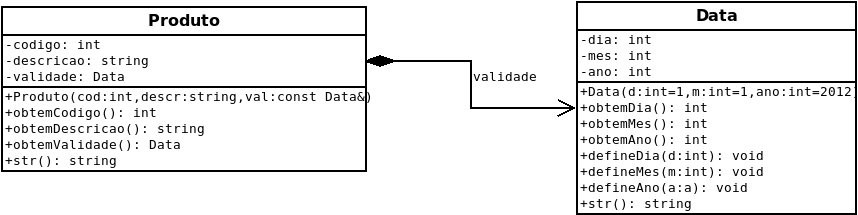
\includegraphics[height=0.40\paperheight]{imagens/modelagem_produto_data.png}
\end{figure}
\end{frame}

%-------------------------------------------------------
\begin{frame}[fragile]\frametitle{Exemplo: Classe Data}
\begin{itemize}
	\item Construtor com parâmetros padrão: importante para utilização dentro de outro objeto
	\item Solução alternativa: construtor sem parâmetro + construtor com parâmetros
\end{itemize}
\begin{columns}[T]
\begin{column}{0.5\linewidth}
\begin{figure}[h]
	\centering
	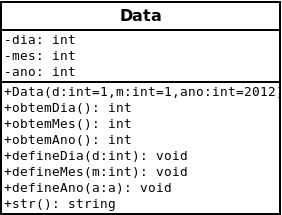
\includegraphics[height=0.40\paperheight]{imagens/modelagem_data.png}
\end{figure}
\end{column}
\begin{column}{0.5\linewidth}
\begin{lstlisting}[basicstyle=\ttfamily\scriptsize]
class Data {
  private:
    int dia, mes, ano;
  public:
    Data(int d=1, int m=1, int a=2012);
    int obtemDia();
    int obtemMes();
    int obtemAno();
    void defineDia(int d);
    void defineMes(int m);
    void defineAno(int a);
    string str();
};
\end{lstlisting}
\end{column}
\end{columns}
\end{frame}

%-------------------------------------------------------
\begin{frame}[fragile]\frametitle{Exemplo: Classe Produto}
\begin{itemize}
	\item Observar o construtor: \texttt{const data \&val}
	\item Indica que o objeto é passado como parâmetro e que \textbf{não} pode ser alterado dentro do construtor
\end{itemize}
\begin{columns}[T]
\begin{column}{0.4\linewidth}
\begin{figure}[h]
	\centering
	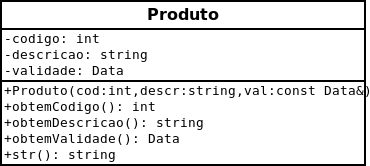
\includegraphics[height=0.25\paperheight]{imagens/modelagem_produto.png}
\end{figure}
\end{column}
\begin{column}{0.6\linewidth}
\begin{lstlisting}[basicstyle=\ttfamily\scriptsize]
class Produto {
  private:
    int codigo;
    string descricao;
    Data validade;
  public:
    Produto(int cod,string descr,const Data &val);
    int obtemCodigo();
    string obtemDescricao();
    Data obtemValidade();
    string str();
};
\end{lstlisting}
\end{column}
\end{columns}
\end{frame}

%-------------------------------------------------------
\begin{frame}[fragile]\frametitle{Exemplo: Programa Principal}
\begin{lstlisting}[basicstyle=\ttfamily\tiny]
#include <iostream>
#include "Data.hpp"
#include "Produto.hpp"

int main() {
  // Cria um objeto Data e ja ajusta os seus atributos
  Data d1(5,5,2007);

  Produto p1(56, "Bolo de Chocolate", d1);

  // Alternativa: cria-se um objeto "anonimo" na propria chamada do construtor

  Produto p2(57, "Bolo de Laranja", Data(12,7,2007));

  // Escreve os dados de p1 e p2
  cout << p1.str() << endl;
  cout << p2.str() << endl;

  return 0;
}
\end{lstlisting}
\begin{itemize}
	\item Compilação:\\
	\texttt{g++ Data.cpp Produto.cpp main.cpp -o programa}
\end{itemize}
\end{frame}

%=======================================================
\section{Lista de Exercícios}

%-------------------------------------------------------
\begin{frame}\frametitle{Lista de Exercícios}
\begin{enumerate}
	\setItemnumber{1}
	\item Criar uma classe \texttt{Automovel} que possui 4 pneus e um motor.
	\\Considere que:
	\begin{itemize}
		\item A classe \texttt{Automovel} possui uma marca, uma quilometragem atual, uma referência para motor e referências para 4 pneus.
		\item A classe \texttt{Pneu} armazena marca e a pressão do ar do pneu.
		\item A classe \texttt{Motor} armazena potência expressa em cavalos (hp), capacidade máxima do tanque de combustível (em litros), nível atual do tanque de combustível (em litros) e consumo médio (em km/l).
	\end{itemize}
	Defina os métodos essenciais para essas classes.\\
	No final, crie um programa principal que instancie um automóvel, contendo um motor e 4 pneus. Sugestão: use a modelagem UML da página a seguir.
\end{enumerate}
\end{frame}

%-------------------------------------------------------
\begin{frame}\frametitle{Modelagem UML para a classe \texttt{Automovel}}
\begin{figure}[h]
	\centering
	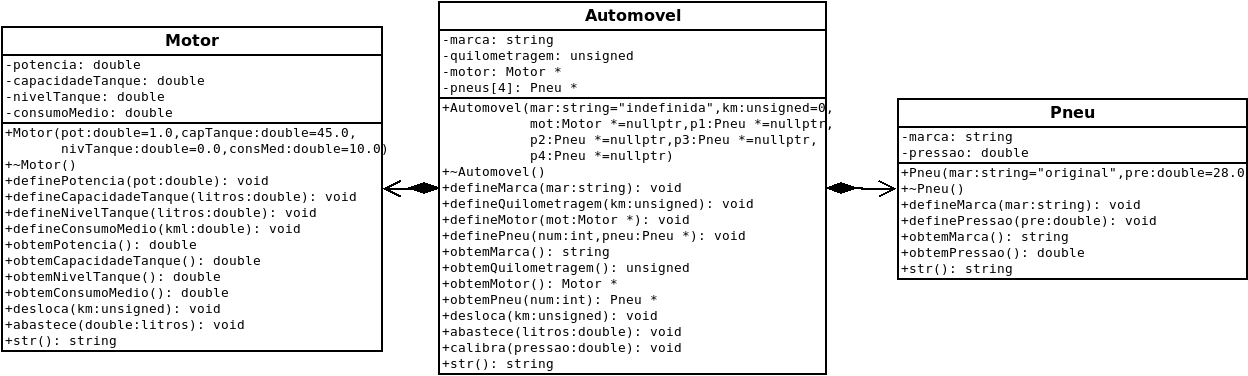
\includegraphics[height=0.45\paperheight]{imagens/modelagem_automovel.png}
\end{figure}
\end{frame}

%-------------------------------------------------------
\begin{frame}[fragile]\frametitle{Lista de Exercícios}
\begin{enumerate}
	\setItemnumber{2}
	\item Faça um programa em C++ que contenha uma classe que representa um funcionário, registrando seu nome, salário e data de admissão. Crie por último uma classe que representa uma empresa, registrando seu nome e CNPJ. Em todas as classes defina os atributos como privados e crie métodos públicos para acessar e modificar os atributos.\\
	Finalmente, faça um programa que:
	\begin{itemize}
		\item Crie uma empresa.
		\item Adicione a empresa alguns funcionários (solicitar no início quantos).
	\end{itemize}
\end{enumerate}
\end{frame}


%=======================================================
\section{Créditos}

%-------------------------------------------------------
\begin{frame}\frametitle{Créditos}
\begin{itemize}
	\item Estas lâminas contêm trechos de materiais disponibilizados pelos professores Rafael Garibotti e Edson Moreno.
\end{itemize}
\end{frame}

%-------------------------------------------------------
\end{document}

